

\documentclass[a4paper,12 pt]{article}
\usepackage{graphicx}
\usepackage{caption}
\usepackage{refstyle}
\usepackage{wrapfig}
\usepackage{subcaption}
\usepackage{geometry}
 \geometry{
 a4paper,
 total={210mm,297mm},
 left=30mm,
 right=30mm,
 top=30mm,
 bottom=30mm,
 }


\title {Project Report \\ Sensor Module Interfacing \\[10pt] Task:
Interfacing PIR Sensor with ATmega2560 in Firebird V Robot \\[25pt] Team members }
\author {Chayatan \and Mukilan A \and Shantanu}

\begin{document}
\maketitle
\begin{center}
\begin{large}
Under the guidance of\\
\textbf{Prof. Kavi Arya\\and\\Parin Chedda}\\
\vspace{0.5in}
\end{large}
\end{center}
\begin{center}

\includegraphics[scale=0.32]{iitb.png}
\end{center}
\begin{center}
\begin{large}
Embedded and Real-Time Systems Laboratory \\
Department of Computer Science and Engineering \\
Indian Institute of Technology \\
Bombay \\
\end{large}
\end{center}

\newpage
\tableofcontents
\newpage

\begin{abstract}
The project aims at interfacing a PIR sensor with Fire Bird
V educational robot. This additional module can be used for detection
of Human Movement. This will
include the detailed explanation of the components of PIR Sensor, its working principle, basic interfacing circuit, programming and
applications.
\end{abstract}
\section{Introduction} 
\vspace {5 mm}
\begin{figure}[h]
\begin{center}
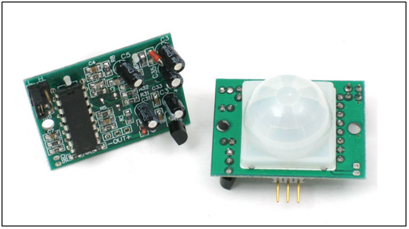
\includegraphics[]{PIR_Sensor.png}
\caption{PIR Sensor Bottom view (left) and Top View (Right)}
\label{fig:1}
\end{center}
\end{figure}
\vspace{-20 pt}
 Passive Infrared Sensors (as shown in \figref{1}) also known as PIR Motion Detector Sensor, is an electronic sensor that measures Infrared (IR) light radiating from objects in its field of view. PIR sensors allow you to sense motion, almost always used to detect whether a human has moved in or out of the sensors range. They are small, inexpensive, low-power, easy to use and don't wear out. For that reason they are commonly found in appliances and gadgets used in homes or businesses. They are often referred to as PIR, "Passive Infrared", "Pyroelectric", or "IR motion" sensors.


\begin{figure}[h]
\begin{center}
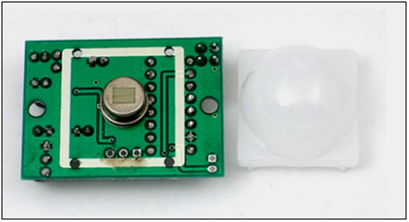
\includegraphics[]{PIR_Sensor_2.png}
\caption{PIR Sensor after removing the plastic casing}
\label{fig:2}
\end{center}
\end{figure}

PIRs are basically made of a pyroelectric sensor which can be seen as the round metal can with a rectangular crystal in the center, as seen in \figref{2} which can detect levels of infrared radiation. Everything emits some low level radiation, and the hotter something is, the more radiation is emitted. The sensor in a motion detector is actually split in two halves.  The two halves are wired up so that they cancel each other out. If one half sees more or less IR radiation than the other, the output will swing high or low. 

\subsection{Specifications}
\begin{itemize}
\item Single bit output
\item Small size makes it easy to conceal
\item Sensitivity: Pre-settable
\item Size: Length 32mm, Width 24mm, Thickness 26mm

\end{itemize}

\section{Components of a PIR Sensor}
\vspace {5 mm}
\begin{figure}[h]
\begin{center}
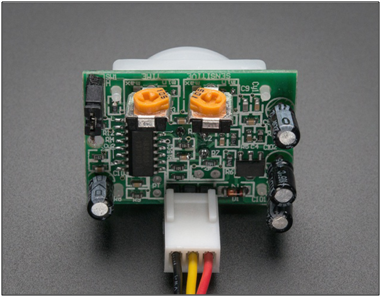
\includegraphics[]{PIR_Sensor_pins.png}
\caption{PIN Connections of a PIR Sensor}
\label{fig:3}
\end{center}
\end{figure}


\large The most important 3 pins of a PIR Sensor:

\begin{itemize}
\item \textbf{+V :} This pin of the PIR sensor should be connected to an external 5V supply. (The red wire as can be seen in \figref{3})
\item \textbf{GND :} This pin of the PIR sensor should be connected to an Ground.(The black wire as can be seen in \figref{3})
\item \textbf{OUT :} This pin of the PIR sensor is the digital output. This pin is to be read by the nicrocontroller to detect the movement and decide the appropriate action that should be taken.(The yellow wire as can be seen in \figref{3})
\end{itemize}
\begin{figure}[h]
\begin{center}
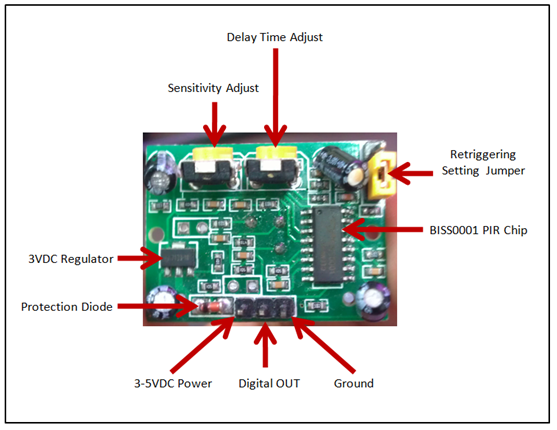
\includegraphics[]{PIR_Sensor_3.png}
\caption{Detailed Diagram of Bottom View of a PIR Sensor}
\label{fig:4}
\end{center}
\end{figure}
%-----------------------------------------------------------------------------
The major components behind the PIR Circuitry and operation are as shown in \figref{4}. These are explained in detailied as follows:

\begin{itemize}
\item \textbf{BISS0001 Chip :} This is the decoder chip, which is used to process the analog signal obtained by the Pyroelectric sensor to give the digital output.
\item \textbf{Protection Diode :} This diode is used in a circuit to protect the circuit from reverse voltage and current.
\item \textbf{3V DC Regulator :} The output generated by the PIR sensor is in the form of digital pulses (3 V), when movement is detected and 0V when no movement detected. To ensure a constant suppy of 3V for the output generated for motion detection, a 3V DC regulator is used.
\end{itemize}


\begin{figure}[h]
\begin{center}
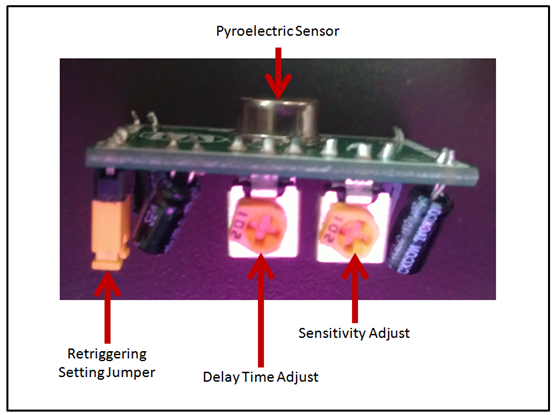
\includegraphics[scale=0.7]{sens.png}
\caption{Detailed Diagram of Side View of a PIR Sensor}
\label{fig:5}
\end{center}
\end{figure}
\begin{itemize}
\item \textbf{Delay Time Adjust :} The trimpot labelled in the \figref{5} is used to adjust the two timeouts available in the PIR Sensor. First timeout is Tx, which is used to indicate the duration the LED is lit after detecting movement and the second timeout is Ti, which is the duration for which the LED would remain off when it detects no movement.
\item \textbf{Sensitivity Adjust :} The trimpot labelled in the \figref{5} is used to adjust the sensitivity. This can be used to increase or decrease the sensitivity. Clockwise turning of the trimpot makes the PIR more sensitive.
\end{itemize}

\begin{figure}[h]
        \centering
        \begin{subfigure}[b]{0.45\textwidth}
                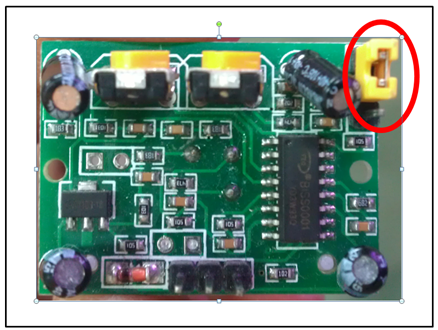
\includegraphics[width=\textwidth]{H.png}
                \caption{ H Jumper Setting for Retrigger Mode}
                \label{fig:6a}
        \end{subfigure}%
        ~ %add desired spacing between images, e. g. ~, \quad, \qquad, \hfill etc.
          %(or a blank line to force the subfigure onto a new line)
        \begin{subfigure}[b]{0.45\textwidth}
                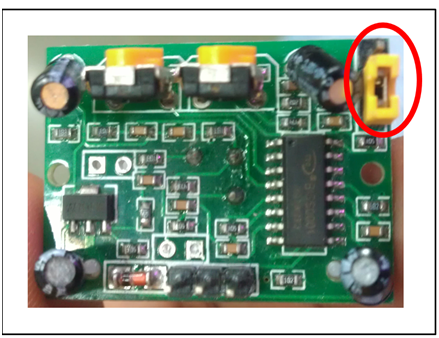
\includegraphics[width=\textwidth]{L.png}
                \caption{L Jumper Setting for Normal Mode}
                \label{fig:6b}
        \end{subfigure}
        
\end{figure}

\begin{itemize}
\item \textbf{Triggering Modes :} There are two triggering modes available in the PIR Sensor

\begin{itemize}
\item \textbf{H Retrigger Mode: }
Output remains HIGH when sensor is retriggered repeatedly. Output is LOW when idle ie not triggered, (as can be seen in \figref{6a})

\item \textbf{L Normal Mode:}
Output goes HIGH then LOW when triggered. Continuous motion results in repeated HIGH/ LOW pulses. Output is LOW when idle (as can be seen in \figref{6b})
\end{itemize}
\end{itemize}
%-----------------------------------------------------------------------------

\section{Working of PIR Sensor} 

\begin{figure}[h]
\begin{center}
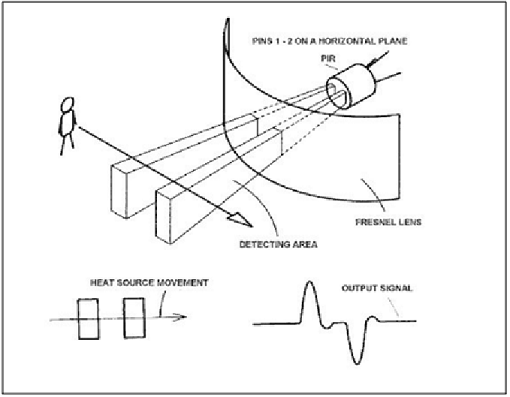
\includegraphics[]{working.png}
\caption{Working of a PIR Sensor}
\label{fig:7}
\end{center}
\end{figure}


The PIR sensor has two slots in it. And each slot is made of a special material that is sensitive to IR. The lens used here is not really doing much and so we see that the two slots can 'see' out past some distance (basically the sensitivity of the sensor). When the sensor is idle, both slots detect the same amount of IR, the ambient amount radiated from the room or walls or outdoors. When a warm body like a human or animal passes by, it first intercepts one half of the PIR sensor, which causes a positive differential change between the two halves of the PIR Sensor. When the warm body leaves the sensing area, the reverse happens, whereby the sensor generates a negative differential change. These change pulses are what is detected.
\pagebreak
\begin{figure}[h]
        \centering
        \begin{subfigure}[b]{0.45\textwidth}
                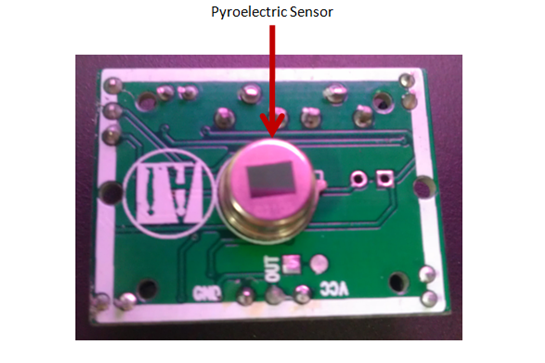
\includegraphics[width=\textwidth]{pyr.png}
                \caption{ Top View of a PIR Sensor (Without Plastic Cover)}
                \label{fig:8a}
        \end{subfigure}%
        ~ %add desired spacing between images, e. g. ~, \quad, \qquad, \hfill etc.
          %(or a blank line to force the subfigure onto a new line)
        \begin{subfigure}[b]{0.45\textwidth}
                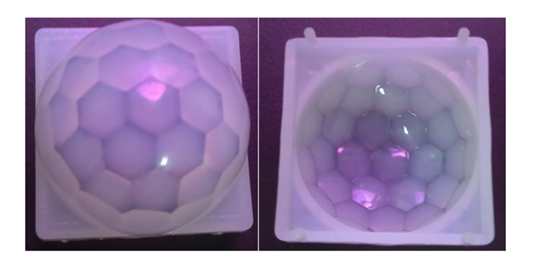
\includegraphics[width=\textwidth]{pyr1.png}
                \caption{Plastic Cover. You can observe the Fresnel lenses inside the Plastic Covering}
                \label{fig:8b}
        \end{subfigure}
        
\end{figure}

\hspace{-7mm}{\textbf{Why an additional platic covering is used on top of the pyroelectric sensor???}}\\
Looking closely at the plastic casing in \figref{8b}, you will observe that the plastic covering is shaped in the form of a bee-hive like structure. Each of the segments in the bee-hive structure is a Fresnel Lens. This Fresnel Lens Array is used to capture more irradiation and focus it to a relatively smaller point. It condenses the light, thus providing a larger range of IR to the sensor.

\pagebreak
\section{Connecting the PIR Sensor to the Firebird V Robot}



\begin{figure}[h]
\begin{center}
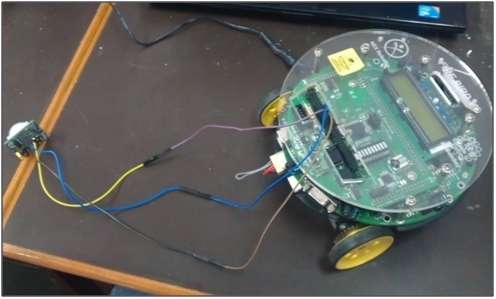
\includegraphics[scale=0.8]{con1.png}
\caption{Connecting the PIR sensor with the Firebird V Robot}
\label{fig:9}

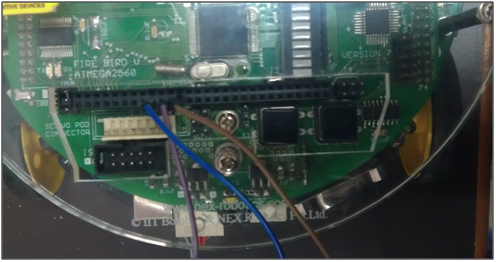
\includegraphics[scale=0.8]{con2.png}
\caption{Connections in the Microcontroller Board Expansion Socket}
\label{fig:10}
\end{center}
\end{figure}


\subsection{Steps to connect PIR Sensor to the Robot:}
\begin{enumerate}
\item 	Connect the GND, +V and the Digital Output pins to the pins in the Firebird V Robot as mentioned in Table 1
\item 	After connecting, read the value of the Digital Output Pin of the FireBird V Robot.
\item 	The output can either be Logic HIGH or LOW, since the output of the PIR Sensor is digital in nature.
\item 	Using these values, you can switch ON or OFF an LED or Buzzer to indicate the presence of a Human. 
\end{enumerate}

\subsection{Pin Connections between PIR Sensor and FireBird V Robot}

\begin{table}[ht]
\hspace{-10mm}
\caption{}
\begin{tabular}{|c|c|}

\hline

$Pins of PIR Sensor$&$Pins of ATmega2560  Microcontroller $\\
$ $&$Board Expansion Socket$\\
\hline
GND&Pin 23/24 (Ground)\\
\hline
+V&Pin 21/22 (5 Volts)\\
\hline
Digital Output&Any Port Pins except the ones used for\\
 &LCD or Bargraph as it is used to display the output\\
\hline
\end{tabular}
\label{table:t1}
\end{table}

\section{C Code}
\subsection{Using the Header File}
A header file has been provided called as 'scan\_pir.h' in the \textbf{Headers} Folder.
It contains the function
\begin{center}
 \textbf{scan\_pir()};
\end{center}
This function is used to read the PIR Sensor digital output and according to the ouput generated, it will display the corresponding output on the Bargraph LEDs and the LCD.\\

\vspace{5mm}\hspace{-8mm} When the PIR output is HIGH, the Bargraph LEDs would switch ON and LCD would display "Human Detected".\\
When the PIR output is LOW, the Bargraph LEDs would switch OFF and LCD would display "Empty Space".\\
\newpage
\subsection{Sample code calling scan\_pir.h header file and scan\_pir() function}
Now we will see the Sample Program calling the scan\_pir.h header file calling the scan\_pir() function. Prior to the C Code. The following connections should be made:
\begin{enumerate}
\item PIR Ground pin must be connected to the Firebird V Ground pin.
\item PIR +V pin must be connected to the Firebird V 5Volts pin.
\item PIR Digital Output Pin must be connected to the Firebird V Port L Pin 6, i.e. Pin 18 in the microcontroller expansion slot.
\end{enumerate}

\begin{center}

\LARGE{\textbf{SAMPLE CODE}}
\end{center}
\begin{verbatim}
#define F_CPU 14745600

#include <avr/io.h>
#include <avr/interrupt.h>
#include <util/delay.h>
#include "scan_pir.h"

//Main Function
int main(void)
{
scan_pir();				//Function to scan the PIR Sensor when the 
            //PIR Digital Output pin is connected to
            //the PORT L Pin 6


            //if the output is HIGH, then the LCD will 
            //display "Human Detected" and the Bargraph
            //LEDs will be ON
            //if the output is LOW, then the LCD will display
            // "Empty Space" and the Bargraph LEDs will be OFF
}

\end{verbatim}

\Large{\textbf{Important Note}}
\large
\begin{enumerate}
\item While running this program you dont need to initialise the PORT Pins for PIR, Bargraph LEDs, and LCD, because Ports have already been configured in the header file where PIR, Bargraph LEDs and LCD have been configured to PORT L, PORT J and PORT C respectively.
\item You need not include the lcd.h header file separately for any other program, because the header file itself calls the lcd.h file to display its output on the LCD screen. But ensure that you have both the scan\_pir.h and lcd.h inside the folder containing your C Code.
\end{enumerate}
\newpage
\subsection{Initialisation of PORT Pins}
\textbf{PIR Port Pins}
\begin{verbatim}
void PIR(void)
{
	DDRL &= ~(1<<PL6);  	 //Setting the direction registers
                      //to make PL6 Pin as INPUT
	PORTL |= (1 << PL6);  //Setting the Port L PIN 6 as Floating
}
\end{verbatim}
 \textbf{Bargraph LED}
\begin{verbatim}
void LED(void)
{
DDRJ = 0xFF;        //Set all the Pins of PORTJ as output port
PORTJ = 0xFF;       //Set all the Pins of PORTJ as logic HIGH
}
\end{verbatim}


\subsection{Main Program}
\begin{verbatim}
int main(void)
{

	unsigned char x;
	int flag=1;
	
	init_devices();             //Initialize all the devices
	lcd_set_4bit();             //Set the LCD in 4 bit mode
	
	while(1)
	{
		
		x = PINL & (1<< 6);        //Read the PL6 pin to read the
                           //PIR Sensor output
		lcd_init();                //Initialize the LCD
		if(x)                      //Check if the PL6 pin is HIGH  
		{
			PORTJ = 0xFF;              //Turn ON Bargraph LED
			
			
			
			if(flag ==1)            //A flag has been added to stop
                        //the screen from re-initializing
                        //every time in the while loop
                        //The Screen initialises only
                        //if changing from Human Detected
                        //Empty Space in LCD
			{
				lcd_init();
				lcd_cursor(1,1);
				
			}
			lcd_string("Human Detected");          //Display "Human Detected"
                                       //on the LCD
			flag=0;
		}
		else
		{
			
			PORTJ = 0x00;                      //Turn OFF Bargraph LED
			
			if(flag==0)
			{
				lcd_init();
				lcd_cursor(1,1);
			}
			lcd_string("Empty Space");         //Display "Empty Space"
                                   //on the LCD
			flag=1;
		}
		
	}
}

\end{verbatim}
\newpage
\section{Sample Output Displayed on the LCD and BarGraph LEDs}
\begin{figure}[h]
        \centering
        \begin{subfigure}[b]{0.45\textwidth}
                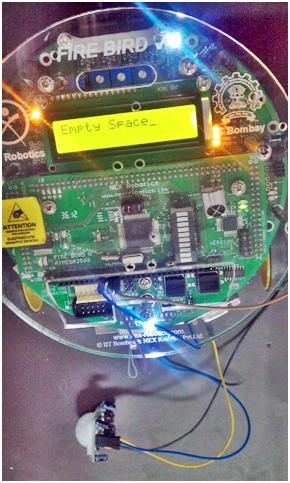
\includegraphics[width=\textwidth]{out1.png}
                \caption{Absence of Human Motion}
                \label{fig:9a}
        \end{subfigure}%
        ~ %add desired spacing between images, e. g. ~, \quad, \qquad, \hfill etc.
          %(or a blank line to force the subfigure onto a new line)
        \begin{subfigure}[b]{0.45\textwidth}
                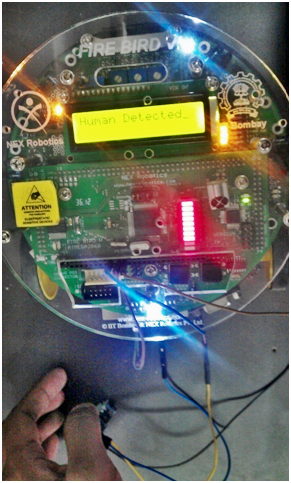
\includegraphics[width=\textwidth]{out2.png}
                \caption{Presence of Human Motion}
                \label{fig:9b}
        \end{subfigure}
        
\end{figure}

The Atmega2560 is interfaced with the LCD as well as the Bar Graph LEDs to display the output as to whether a human motion is detected or not.
\begin{itemize}
\item \textbf{When motion is absent:}
The LCD displays “Empty Space” and the Bargraph LEDs are switched OFF, as can be seen in  \figref{9a})

\item \textbf{When motion is present:}
The LCD displays “Human Detected” and the Bargraph LEDs are switched ON as can be seen in \figref{9b})
\end{itemize}
\pagebreak

\section{Applications}
\begin{itemize}
\item \textbf{Human Detection Applications : }\\
PIR Sensor on detecting a human body generates a HIGH Pulse. This application is useful for automatic doors, security systems, Medical purposes, Surveillance and Civil Applications.

\item \textbf{Thermal Imaging :}\\
PIR sensors can be used to detect the thermal radiation of the object with great accuracy and precision. This can be used in thermal imaging, which finds its applications in security services such as airport customs control, fire department, industries for detecting heat leakages and in military applications. \textit{ This can also be used in Rescue missions during earthquakes, such that the PIR sensor in drones will detect the presence of humans under the debris, so that appropriate rescue operation can be carried out.}

\item \textbf{Infrared Homing :}\\
This application takes place in the missile guiding system. The tracking system works with the emitted electromagnetic radiation from the target. Target tracking is connected to heat radiation detection.
\end{itemize}

\newpage
\begin{center}
\section*{References}
\end{center}
\vspace{20mm}
\begin{itemize}
\item PIR Motion Sensor, available at:
\begin{verbatim}
 https://learn.adafruit.com/pir-passive-infrared-proxi-
 mity-motion-sensor/overview
\end{verbatim}
\item Insight - Learn the Working of a Motion Sensor or PIR Sensor, available at:
\begin{verbatim}
 http://www.engineersgarage.com/insight/how-motion-pir-
 sensor-works
\end{verbatim}

\item PIR Motion Detection Sensor - Nex Robotics, \\available at: 
\begin{verbatim}
http://www.nex-robotics.com/images/downloads/pir_sens-
or.pdf
\end{verbatim}

\item PIR  Sensor - Instructions, Limitations and Sample Applications, \\available at: 
\begin{verbatim}
http://www.egr.msu.edu/classes/ece480/capstone/fall09/g-
roup05/docs/ece480_dt5_application_note_bseracoglu.pdf
\end{verbatim}
\end{itemize}
\end{document}